As early as 1964, Goffman~\cite{goffman64OnRelevanceAsAMeasure}, a
mathematical information science pioneer \cite{harmon08RememberingWG},
notes that the relevance of documents in a list has to depend on the
documents preceding it.  More recently, work on
MMR~\cite{carbonell98MMR} was one of the first to formalize
diversification as a mathematical optimization criterion; MMR has
proved one of the most popular diversity approaches.  Aside from this
work, two of the other notable works are~\cite{yue081224Predicting},
which formalizes a structured SVM loss function based on a set
covering objective, and~\cite{wang09PortfolioTheory}, which borrows
concepts from portfolio theory in economics to treat result set
diversification as optimization of a risk minimization objective.  We
note that the results as derived in the last section formally motivates these
last three somewhat ad-hoc diversification approaches and we discuss
these connections more deeply in the following sections.


%\subsection{MMR}
%
%The result in~\eqref{eq:1call} is strikingly similar to MMR --- it
%contains two terms, one for query similarity and the other for result
%set diversification, where each term represents a similarity kernel
%--- more specifically a \emph{probability product kernel}
%(PPK)~\cite{prodprobkernel} that is an inner product of probability
%vectors (or more generally, functions).  More formally, let
%$\vec{T}'$, $\vec{T}_k$, and $\vec{T}_{S_{k-1}^*}$ be respective topic
%probability vectors $P(t'=t|\vec{q})$, $P(t_k=t|s_k)$ and
%$\tilde{P}(t_k=t | S_{k-1}^*)$ with vector indices for each topic $t
%\in T$.  Then the similarity and diversity terms from~\eqref{eq:1call}
%can be respectively written as
%\begin{align}
%%\Sim_1(\vec{q},s_k) = & \hspace{-3mm}
%\sum_{t \in T} P(t'=t|\vec{q}) P(t_k=t|s_{k}) & \; = \; \langle \vec{T}',\vec{T}_k \rangle \label{eq:sim_term} \; \mbox{and}\\
%%\Sim_2(s_k,S_{k-1}) = & \hspace{-3mm}
%\sum_{t \in T} P(t|\vec{q}) P(t_k=t|s_k) \tilde{P}(t | S_{k-1}^*) & \; = \; \langle \vec{T}_k, \vec{T}_{S_{k-1}^*} \rangle_{\vec{T}'}. \label{eq:div_term}
%\end{align}
%Here, we let $\langle \cdot,\cdot \rangle$ denote an inner product of
%two vectors and $\langle \cdot,\cdot \rangle_\vec{v}$ a
%\emph{$\vec{v}$-reweighted} inner product, defined as
%in~\eqref{eq:div_term}.
%
%While having similarity and diversity terms similar to MMR,
%Exp-$1$-call@$k$ in~\eqref{eq:1call} clearly differs from MMR:
%\begin{enumerate}
%\item While MMR's definition allows for any similarity function, not
%just PPKs, we note that \emph{equating words to subtopics}, popular
%kernels like TF and TFIDF~\cite{salton83Introduction} can be viewed
%directly as PPKs if the TF and TFIDF vectors are $L_1$ normalized to
%represent probability vectors.
%\item MMR uses a maximization term for
%diversity, whereas optimization of Exp-$1$-call@$k$ instead calls for
%a product (noisy-or) diversity term $\tilde{P}(t | S_{k-1}^*)$.
%We note that a noisy-or reduces to a max when the subtopic
%probabilities are deterministic (0 or 1).
%\item While MMR proposes a $\lambda$ term to explicitly
%trade off the similarity and diversity terms, the greedy optimization
%of Exp-$1$-call@$k$ in~\eqref{eq:1call} yields no such trade-off term
%(or alternately, an implicit $\lambda=.5$).  Although it seems a tunable
%$\lambda$ is not needed for maximizing Exp-$1$-call@$k$, it may be
%desirable when maximizing surrogate retrieval objectives (e.g., ranking
%objectives).
%\item Optimizing Exp-$1$-call@$k$ introduces query-specific relevance into
%the diversification term as shown
%by the query topic ($\vec{T}'$) reweighted
%diversity function in~\eqref{eq:div_term}.
%\end{enumerate}
%
%%To verify whether the differences between MMR and Exp-$1$-call@$k$
%%matter empirically, we compare the two algorithms across a number of
%%metrics on three diversity testbeds: the TREC 6-8 Interactive
%%Track\footnotemark[1] (17 queries) and 2009 and 2010 ClueWeb Diversity
%%tasks of the TREC Web Track\footnotemark[2] (50 queries each).  On
%%these testbeds, we evaluate \emph{mean subtopic
%%recall@$k$}~\cite{zhai03Beyond} (fraction of total annotated
%%aspects/subtopics covered by a result set at rank $k$, averaged over
%%queries), which is an appropriate loss function for the
%%\emph{set-level} metric~\eqref{eq:setRelevance}~\cite{chen06Less}.  We
%%also evaluate a variety of more recent \emph{rank-based} diversity evaluation
%%metrics such as intent-aware expected reciprocal rank
%%(ERR-IA@$k$)~\cite{err-ia}, $\alpha$-nDCG@$k$~\cite{clarke08Novelty},
%%and intent-aware mean average precision
%%(MAP-IA)~\cite{agrawal09diversifying}.
%%
%%We use MMR with $\lambda = 0.5$ to match the equal weighting of
%%similarity and diversity in Exp-$1$-call@$k$.  An
%%LDA~\cite{blei03Latent} topic model is trained on the top-100 OKAPI
%%BM25~\cite{bm25} results for each query (on its respective collection)
%%and these subtopic distributions are used for the similarity and
%%diversity kernels in both algorithms: for MMR we choose $\Sim_1$ and
%%$\Sim_2$ kernels as in~\eqref{eq:sim_term} --- effectively LDA
%%variants of latent semantic indexing (LSI)~\cite{deerwester90LSA}
%%kernels; for Exp-$1$-call@$k$, we use the similarity and diversity
%%kernels respectively defined in~\eqref{eq:sim_term}
%%and~\eqref{eq:div_term}.  Both MMR and Exp-$1$-call@$k$ are used to
%%rank the top-20 documents from the top-100 OKAPI BM25 results.
%%
%%Results in Table~\ref{table:different_metrics} and
%%Figure~\ref{fig:mmr_vs_1call} show the performances of MMR and
%%Exp-$1$-call@$k$ on the three diversity testbeds across various
%%diversity measures; although there are minor performance differences,
%%we note that these differences are not statistically significant
%%w.r.t.\ 95\% confidence intervals.  Nonetheless, the results appear to
%%indicate that the structural similarities in the use of MMR and the
%%optimization of Exp-$1$-call@$k$ outweigh the differences in this
%%evaluation.
%
\subsection{Relations of Exp-$1$-call@$k$ and Other Diversification Approaches}

Recent years have seen numerous proposals for diversification
approaches and here we summarize the relationship between optimization
of Exp-$1$-call@$k$ and representatives of these alternative
approaches:

\subsubsection{Diversifying Search Results}
\cite{agrawal09diversifying} proposes a set-based objective function
to answer ambiguous web queries in a setting where there exists a predefined taxonomy of information, and that both queries and documents
may belong to more than one category according to this taxonomy. The proposed set-based objective function aims at maximizing the probability that the average user finds at least one useful resulting document retrieved within the top $k$ results. Mathematically, this objective function is defined below:
\begin{align}
	P(S_k|\vec{q}) = \sum_{t\in T} P(t|\vec{q}) \left( 1 - \prod_{i=1}^{k}(1-p(t_i = t| q, s_i))\right) 
\label{eq:diversifykObjectiveFunction}
\end{align}
Note first that we have adapted notations in the above equation for consistency, and note also that the taxonomy $P(t|\vec{q})$ and $P(t_i|s_i)$ are not learnt by some unsupervised model, but hand-crafted. 

Now we show that our expected 1-call@$k$ objective in Equation~\eqref{eq:setRelevance} is equivalent to the objective function in Equation \eqref{eq:diversifykObjectiveFunction} by simply writing out the mathematical expectation in terms of the sum over all possible topics (e.g., taxomony in \cite{agrawal09diversifying}) the weighted relevance where weights are the topic distributions below
\begin{align*}
    \ExpOneCall(S_k,\vec{q}) & = \mathbb{E} \left[\left. \bigvee_{i=1}^{k}r_i=1 \right| s_{1},\dots, s_{k},\vec{q} \right], \\
    												 & = \sum_{t\in T} P(t|\vec{q}) \left( 1 - \prod_{i=1}^{k}(1-p(t_i = t| q, s_i))\right) 
\end{align*}
Our observation here is that the proposed objective in \cite{agrawal09diversifying} is equivalent to our objective, however they do not derive this from the expected 1-call@$k$ objective.

\subsubsection{Portfolio Theory}
\cite{wang09PortfolioTheory} motivates
diversification in set-based information retrieval by a
risk-minimizing portfolio selection approach.  Viewing a result set as
an investment portfolio with the objective to maximize return while
minimizing risk, the derived result of~\cite{wang09PortfolioTheory}
mimics both MMR and Exp-$1$-call@$k$ in that the similarity term may
be viewed as \emph{expected portfolio payoff} (relevance) and the
diversity term may be viewed as \emph{expected portfolio risk}, which
increases as the correlations between documents in the result set
increase.  One major difference in this framework is that rather than
computing the diversity term via a max (MMR) or product
(Exp-$1$-call@$k$) the portfolio theory derivation uses a summation
--- we examine the implications of this next.

\subsubsection{Set Covering:}
Yue and Joachims~\cite{yue081224Predicting} propose a set covering
approach for training SVMs to predict diverse result sets for
information retrieval.  In their work, they equate subtopics with
words and build a loss function for SVM training that penalizes
result sets according to the sum of weights of query-relevant words
\emph{not} covered by the result set.  While their approach provides a
``hard'' set-covering view of diversity, we note that an expansion of
$\tilde{P}(t | S_{k-1}^*)$ used in the diversity term
of~\eqref{eq:1call} provides a ``soft'' latent set-covering
interpretation; that is, $s_k$ is chosen so as to best cover (in a
probabilistic sense) the latent topic space not already covered by $\{
s_1^*,\ldots,s_{k-1}^* \}$.  Formally, expanding the product in
$\tilde{P}(t | S_{k-1}^*) = \prod_{i=1}^{k-1} \left(1 -
P(t_{i}=t|s_{i}^{*})\right)$, collecting terms and writing it as a
series, we arrive at a form that reflects the inclusion-exclusion
principle applied to the calculation of probability that topic $t$ is
covered by $\{ s_1^*,\ldots,s_{k-1}^* \}$:
\begin{align}
& \prod_{i=1}^{k-1} \left(1 - P(t_{i}=t|s_{i}^{*})\right) \nonumber \\
& = 1 - \left[ \sum_{i=1}^{k-1} P(t_{i}= t|s_{i}^{*}) - \sum_{i=1}^{k-1}\sum_{j=1}^{k-1}P(t_{i}= t|s_{i}^{*})P(t_{j}= t|s_{j}^{*}) \right. \nonumber \\
& \hspace{12mm} \left. + \dots - (-1)^{k-1}\prod_{i=1}^{k-1}P(t_{i}=t|s_{i}^{*})\right] \label{eq:setcover}
\end{align}

This result has a natural interpretation: the first summation term
determines the coverage of topic $t$ by each document $s_i$ ($1 \leq i
\leq k-1$) currently in the result set, the second double summation
term corrects the first term by removing the joint probability mass
from all pairs of documents that was double counted, and so on
according to the principle of inclusion-exclusion.
\eqref{eq:setcover} not only provides a probabilistic set covering
view of Exp-$1$-call@$k$, but it also suggests that a portfolio
approach to diversity using only the first summation would overcount
each document's contribution to the diversity metric according to this
set covering perspective.

The inclusion-exclusion principle calculation provided by the second term in Equation~\ref{eq:setcover}
is illustrated in~Figure~\ref{fig:inclusionExclusionPrinciple}. In words, this term is calculating the total topic probability coverage of $t$ by all
selected items $\{ s_1^*,\ldots,s_{k-1}^* \}$ by properly applying the
inclusion-exclusion principle to ensure that overlapping probability coverage
is not double counted. Then referring back to Equation~\ref{eq:partial_simp}, we note that $s_k$ is chosen by maximizing a weighted
sum over topics, where each topic weight is determined by its relevance
to the query $\vec{q}$, the item $s_k$, and penalized (i.e., due to the $1 - $)
by the topic coverage of $t$ by the set $\{ s_1^*,\ldots,s_{k-1}^* \}$ to
naturally encourage diversity.  We note that this is a soft probabilistic
version of the ``in or out'' topic coverage approach of WSL.

%%%%%%%%%%%%%%%%%%%%%%%%%%%%%%%%%%%%%%%%%%%%%%%%%%%%%%%%%%%%%%
\begin{figure}[t!]
\begin{center}
\centerline{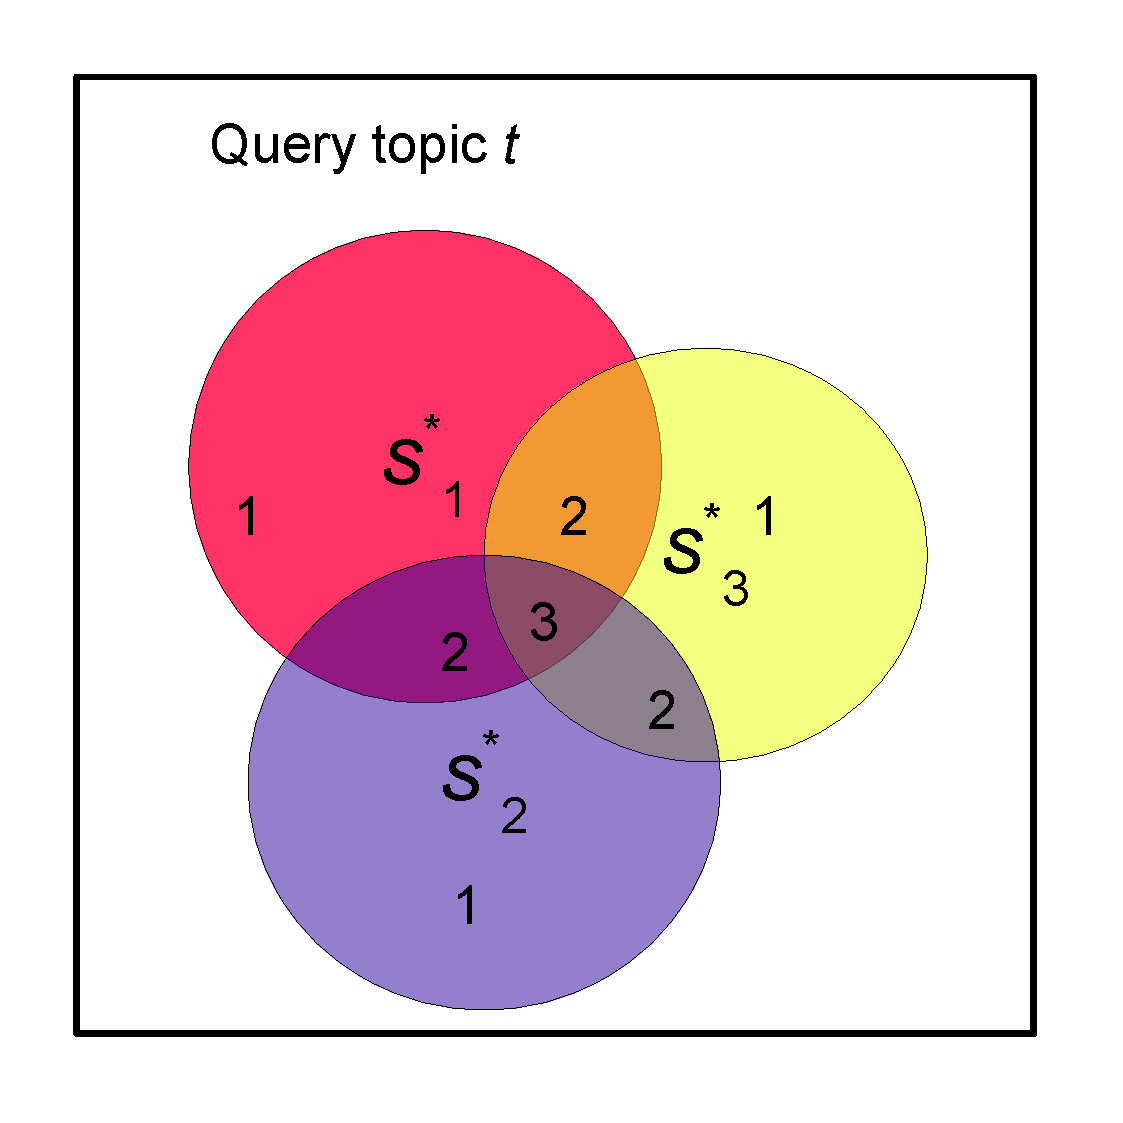
\includegraphics[scale = 0.4]{inclusionExclusionPrinciple}}
\caption[Inclusion-exclusion principle.]{Inclusion-exclusion principle. The sets represent candidate
items $s$ for a query, and the area covered by each set is the
``information" covered by that item for query topic $t$. Numbers on different areas
indicates the number of sets that share these areas. }
\label{fig:inclusionExclusionPrinciple}
\end{center}
\end{figure}
%%%%%%%%%%%%%%%%%%%%%%%%%%%%%%%%%%%%%%%%%%%%%%%%%%%%%%%%%%%%%%

\subsubsection{Subtopic Relevance Models} 
We use a subtopic relevance
model that is a simplified version of the model in~\cite{plmmr} with
fewer dependence assumptions.  In other work, Zhai {\it et
al}~\cite{zhai03Beyond} present an empirical risk minimization view of
dependent document retrieval from a subtopic perspective,
where they derive a formalization of the
\emph{greedy} selection step that is similar to MMR and to a lesser
extent, Exp-$1$-call@$k$.

\subsubsection{Set-based Relevance Objectives} 
Chen and Karger~\cite{chen06Less}, whose derivation we extended, directly
optimize $1$-call@$k$, but their intention is not to formalize MMR and
instead use na\"{i}ve Bayes to directly evaluate
\eqref{eq.ncall}.  Agrawal et al~\cite{agrawal09diversifying}
and Santos et al (xQuad)~\cite{santos2010xquad} both specify set-based
diversity metrics \emph{very} similar to Exp-$1$-call@$k$ but do not provide
formal derivations as we have done in this work.

\subsubsection{Ranking Based Objectives} 
Finally, returning to our introductory motivation, Wang and Zhu~\cite{wangzhu10} have shown that
natural forms of result set diversification arise via the optimization
of average precision~\cite{ap} and reciprocal rank~\cite{mrr}.  Both
of these methods share the view of directly optimizing a
\emph{ranking-based} objective, whereas this paper proposes a novel
derivation from the alternate view of optimizing a \emph{set-based}
objective w.r.t.\ a subtopic model of relevance.  However, even though
Exp-$1$-call@$k$ is a set-based objective, an indirect consequence of
(and motivation for) greedily optimizing it is that documents added
earlier yield a greater increase in objective than those added later;
this yields a natural rank ordering on the greedy Exp-$1$-call@$k$
result set.

\subsection{Four Aspects of Diversifying Approaches}
As the last part of the related work, we identify four key aspects for a diversifying approach, and review existing diversifying approaches against these aspects in this section. As shown in Table~\ref{table:comparisonAlgorithms}, we breakdown the
different proposals according to whether they are probabilistic, use
latent models for determining similarity, use adaptive learning
techniques, and finally whether they are unsupervised, i.e., they do
not require labeled data or feedback. We note that our model is the first
proposal (that we are aware of) to combine all four traits in the
affirmative. 

%%%%%%%%%%%%%%%%%%%%%%%%%%%%%%%%%%%%%%%%%%%%%%%%%%%%%%%%%%%%%%%
\begin{table}
\tbl{Dimensions of diversified set-based retrieval
systems: \emph{Probabilistic}: uses probabilistic models?; \emph{Latent}: use
latent topic models?; \emph{Learning}: uses some form of learning?;
\emph{Unsupervised}: does not require labeled topic data or feedback?}{
\begin{tabular}{lcccc}
\hline
Diversity Paper                                    &Probabilistic&  Latent & Learning & Unsupervise  \\
\hline
Carbonell \cite{carbonell98MMR}                    &             &         &         & $\surd$\\
Anagnostop \cite{anagnostopoulos05245Sampling}		 & $\surd$     &         &         & $\surd$\\
Radlinski \cite{radlinski06691Improving}           &             &         &         & $\surd$\\
Radlinski \cite{radlinski08LearningDiverse}        & $\surd$     &         & $\surd$ & \\
Clarke \cite{clarke08Novelty}                      & $\surd$     &$\surd$  &         & $\surd$\\
Yue \cite{yue081224Predicting}                     &             &$\surd$  & $\surd$ & \\
Bai \cite{bai08Adapting}                           &             &         & $\surd$ & $\surd$\\
Sanderson \cite{sanderson08Ambiguous}              &             &         &         & $\surd$\\
Yu \cite{yu09368}                                  &             &         &         & $\surd$\\
Agrawal \cite{agrawal09diversifying}               & $\surd$     & $\surd$ &         & $\surd$\\
Gollapudi \cite{gollapudi09AnAxiomatic}            &             &         &         & $\surd$\\
Clough \cite{clough09734Multiple}                  & $\surd$     &         &         & $\surd$\\
Song \cite{song09Identification}                   & $\surd$     &         & $\surd$ & \\
Wang \cite{wang09PortfolioTheory}                  &             & $\surd$ &         & $\surd$\\
Neal \cite{lathia10TemporalDiversity}              &             &         &         & \\
Zhao \cite{Zhao:SIGIR2012}                         &             &         &         & \\
Dang \cite{Dang:SIGIR2012}                         & $\surd$     & $\surd$ &         & $\surd$ \\
Vargas \cite{Vargas:SIGIR2012}										 & $\surd$     &         & $\surd$ & $\surd$    \\
Our model (this paper)                             & $\surd$     & $\surd$ & $\surd$ & $\surd$ \\
\hline
\end{tabular}}
\label{table:comparisonAlgorithms}
\end{table}
%%%%%%%%%%%%%%%%%%%%%%%%%%%%%%%%%%%%%%%%%%%%%%%%%%%%%%%%%%%%%%%

%\subsection{Temporal Diversification in Recommender Systems}
%Another closely related line of study on diversification applies into recommender systems, thus we discuss these approaches here. 
%\subsubsection{Static Diversification in Recommender Systems}
%
%\subsubsection{Temporal Diversification in Recommender Systems}
